\chapter{Complex Numbers}
By definition a complex number has two parts: a real part and an imaginary part. You already know about real numbers and know about
them. However, imaginary numbers is something different.
\section{Imaginary Numbers}
Imaginary numbers are called so because there cannot be physical representation of these quantities. Like we use real numbers for
counting physical objects we cannot do that with imaginary numbers. In real world, they do not exist. Square root of negative
numbers are called imaginary numbers. For example, $\sqrt{-1}, \sqrt{-2}. \sqrt{-3}, \ldots$ and so on.

We denote $\sqrt{-1}$ with the Greek symbol $\iota$, which stands for \textit{iota}. We also use English letters \textit{i} or
\textit{j} to represent this imaginary number. Clearly, $i^2 = -1, i^3 = -i, i^4 = 1$. If you examine carefully, you will find that
following holds true:

$$i^{4m} = 1, i^{4m + 1} = i, i^{4m + 2} = -1 \text{~and~} i^{4m +3} = -1, \forall m\in P$$

\dangersign \textbf{Gotcha:}

Consider the following:

$$1 = \sqrt{1} = \sqrt{-1*-1} = \sqrt{-1}*\sqrt{-1} = i*i = -1$$

However, the above result is wrong. The reason being is that for any two real numbers $a$ and $b, \sqrt{a}*\sqrt{b} = \sqrt{ab}$
holds good if and only if two numbers are either zero or positive. Also, $\sqrt{1}\neq \sqrt{-1*-1}$ because power of $-$ is
$\frac{1}{2}$ which results in $-1$.

\section{Definitions Related to Complex Numbers}
A complex number is written as $a + ib$ or $x + iy$ or $a + jb$ or $x + jb$. Here, $a, b, x, y$ are all real numbers. The complex
numbers itself is denoted by $z$. Therefore, we have $z = x + iy$. Here, $x$ is called the real part and is also denoted by $Re(z)$
and $y$ is called the imaginary part and is also denoted by $Im(z)$.

A complex number is purely real if its imaginary part or $y$ or $Im(z)$ is zero. Similarly, a complex number is purely imaginary if
its real part or $x$ or $Re(z)$ is zero. Clearly, as you can imagine that there can exist only one number which has both the parts
as zero and certainly that is $0$. That is, $0=0+i0$.

The set of all complex number is typically denoted by $C$. Two complex numbers $z_1$ and $z_2$ are said to be true if there real
parts are equal and imaginary parts are equal. That is if $z_1=x_1+iy_1$ and $z_2=x_2+iy_2$ then $x_1$ must be equal to $x_2$ and
similarly for imaginary part for two complex numbers to be equal.

\section{Simple Arithmetic Operations}
\subsection{Addition}
$(a + ib) + (c + id) = (a + c) + i(b + d)$
\subsection{Subtraction}
$(a + ib) - (c + id) = (a - c) + i(b - d)$
\subsection{Multiplication}
$(a + ib) * (c + id) = ac + ibc + iad + bdi^2 = (ac - bd) +i(bc + ad)$
\subsection{Division}
The complex number in denominator must not have both parts as zero. At least one part must be non-zero.

$$\frac{a + ib}{c + id} = \frac{(a + ib)(c - id)}{(c + id)(c -id)} = \frac{(ac + bd) + i(bc -ad)}{c^2+d^2}$$

\section{Conjugate of a Complex Number}
Let $z = x + iy$ be a complex number then its complex conjugate is a number with imaginary part made negative. It is written as
$\overline{z} = x - iy. \overline{z}$ is the typical representation for conjugate of a complex number $z$.

\subsection{Properties of Conjugates}
\begin{enumerate}
\item $z_1 = z_2 \Leftrightarrow \overline{z_1} = \overline{z_2}$

  Clearly as we know for two complex numbers to be equal, both parts must be equal. So this is very easy to understand that if $x_1
  = x_2$ and $y_1 = y_2$ then this bidirectional condition is always satisfied.
\item $\overline{\left(\overline{z}\right)} = z$

  $z = x + iy$, hence, $\overline{z} = x - iy$. Hence, $\overline{\left(\overline{z}\right)} = x - (-iy) = x + iy = z$
\item $z + \overline{z} = 2Re(z)$

  $z + \overline{z} = x + iy + x - iy = 2x = 2Re(z)$.
\item $z - \overline{z} = 2iIm(z)$

  $z - \overline{z} = x + iy - (x - iy) = 2iy = 2iIm(z)$
\item $z = \overline{z} \Leftrightarrow z$ is purely real.

  Clearly, $x + iy = x - iy \Rightarrow 2iy = 0 \Rightarrow y = 0$. Therefore, $z$ is purely real. Conversely, if $z$ is purely
  real then $z = x$, and thus $z = \overline{z}$.
\item $z + \overline{z} = 0 \Leftrightarrow z$ is purely imaginary.

  Clearly, $x + iy + x - iy = 0 \Rightarrow 2x = 0$. Therefore, $z$ is purely imaginary. Conversely, if $z$ is purely imaginary
  then $z = iy$, and thus $z + \overline{z} = 0$.
\item $z\overline{z} = [Re(z)]^2 + [Im(z)]^2$

  Clearly, $z\overline{z} = (x + iy)(x - iy) = x^2 + y^2 = [Re(z)]^2 + [Im(z)]^2$
\item $\overline{z_1 + z_2} = \overline{z_1} + \overline{z_2}$

  $\overline{z_1 + z_2} = \overline{(x_1 + iy_1) + (x_2 + iy_2)} = \overline{(x_1 + x_2) + i(y_1 + y_2)} = (x_1 + x_2) - i(y_1 +
  y_2) = (x_1 - iy_1) + (x_2 - iy_2) = \overline{z_1} + \overline{z_2}$
\item $\overline{z_1 - z_2} = \overline{z_1} - \overline{z_2}$

  This can be proven like previous item.
\item $\overline{z_1z_2} = \overline{z_1}\overline{z_2}$

  This can be proven like previous item.
\item $\overline{\left(\frac{z_1}{z_2}\right)} = \frac{\overline{z_1}}{\overline{z_2}}$ if $z_2\neq 0$

  It can be proven by multiplying and dividing by conjugate of denominator and then applying division formula given above.
\item If $P(z) = a_0 + a_1z + a_2z^2 + \ldots + a_nz^n$, where $a_0, a_1, \ldots, a_n$ and $z$ are complex numbers, then

  $$\overline{P(z)} = \overline{a_0} + \overline{a_1}(\overline{z}) + \overline{a_2}(\overline{z})^2 +
  \overline{a_n}(\overline{z})^n = \overline{P}(\overline{z})$$

  where

  $$\overline{P}(z) = \overline{a_0} + \overline{a_1}z + \overline{a_2}z^2 + \ldots + \overline{a_n}z^n$$
\item If $R(z) = \frac{P(z)}{Q(z)}$, where $P(z)$ and $Q(z)$ are polynomials in $z$, and$Q(z) \neq 0$, then

  $$\overline{R(z)} = \frac{\overline{P}(\overline{z})}{\overline{Q}(\overline{z})}$$
\item If $$z = \begin{vmatrix}a_1 & a_2 & a_3\\ b_1 & b_2 & b_3 \\ c_1 & c_2 & c_3\end{vmatrix}, \text{~then~}\overline{z}
  = \begin{vmatrix}\overline{a_1} & \overline{a_2} & \overline{a_3}\\ \overline{b_1} & \overline{b_2} & \overline{b_3}
    \\ \overline{c_1} & \overline{c_2} & \overline{c_3}\end{vmatrix},$$
  where $a_i, b_i, c_i(i = 1,2,3)$ are complex numbers.
\end{enumerate}

\section{Modulus of a Complex Number}
Modulus of a complex number $z$ is denoted by $|z|$ and is equal to the real number $\sqrt{x^2 + y^2}$. Note that $|z| \geq
0~\forall z \in C$.
\subsection{Properties of Modulus}
\begin{enumerate}
\item $|z| = 0 \Leftrightarrow z = 0$

  Clearly, this means $x^2 + y^2 = 0 \Rightarrow x = 0$ and $y = 0 \Rightarrow z = 0$.
\item $|z| = |\overline{z}| = |-z| = |-\overline{z}|$

  Clearly, all result in $\sqrt{x^2 + y^2}$.
\item $-|z| \leq Re(z) \leq |z|$.

  Clearly, $-\sqrt{x^2 + y^2}\leq x\leq \sqrt{x^2 + y^2}$.
\item $-|z| \leq Im(z) \leq |z|$.

  Clearly, $-\sqrt{x^2 + y^2}\leq y\leq \sqrt{x^2 + y^2}$.
\item $z\overline{z} = |z|^2$

  Clearly, $(x + iy)(x - iy) = x^2 + y^2 = |z|^2.$
\end{enumerate}

\noindent Following relations are very easy and can be proved by the student. If $z_1$ and $z_2$ are two complex numbers then,

\begin{enumerate}[resume]
\item $|z_1z_2| = |z_1||z_2|$

  $|z_1z_2| = |x_1x_2 - y_1y_2 + i(x_1y_2 + x_2y_1)| = \sqrt{(x_1x_2 - y_1y_2)^2 + (x_1y_2 + x_2y_1)^2} = \sqrt{(x_1 + y_1)^2(x_2 +
  y_2)^2} = |z_1||z_2|$
\item $\left|\frac{z_1}{z_2}\right| = \frac{|z_1|}{|z_2|}$ if $z_2\neq = 0$
\item $|z_1 + z_2|^2 = |z_1|^2 + |z_2|^2 + \overline{z_1}z_2 + z_2\overline{z_2} = |z_1|^2 + |z_2|^2 + 2Re(z_1\overline{z_2})$.
\item $|z_1 - z_2|^2 = |z_1|^2 + |z_2|^2 - \overline{z_1}z_2 - z_1\overline{z_2} = |z_1|^2 + |z_2|^2 + 2Re(z_1\overline{z_2})$.
\item $|z_1 + z_2|^2 + |z_1 - z_2|^2 = 2\left(|z_1|^2 + |z_2|^2\right)$.
\item If $a$ and $b$ are real numbers, and $z_1$ and $z_2$ are complex numbers, then

  $|az_1 + bz_2|^2 + |bz_1 - az_2|^2 = (a^2 + b^2)\left(|z_1|^2 + |z_2|^2\right)$.
\item If $z_1, z_2\neq = 0$, then $|z_1 + z_2|^2 = |z_1|^2 + |z_2|^2 \Leftrightarrow \frac{z_1}{z_2}$ is purely imaginary.
\item If $z_1$ and $z_2$ are complex numbers then $|z_1 + z_2| \leq |z_1| + |z_2|$. This inequality can be generalized to more
  terms as well.
\item $|z_1 - z_2| \leq |z_1| + |z_2|, ||z_1| - |z_2||\leq |z_1| + |z_2|$ and $|z_1 - z_2|\geq ||z_1| - |z_2||$. These are trivial
  to prove.
\end{enumerate}

\section{Geometrical Representation}
A complex number $z$ which we have considered to be equal to $x+iy$ in our previous representations can be represented by a point
$P$ whose Cartesian coordinates are $(x,y)$ referred to rectangular axes $Ox$ and $Oy$ where $O$ is origin i.e. $(0, 0)$ and are
called \textit{real} and \textit{imaginary} axes respectively. The $xy$ two-dimensional plane is also called \textit{Argand plane,
complex plane} or \textit{Gaussian plane}. The point $P$ is also called the image of the complex number and $z$ is also called
the \textit{affix} or \textit{complex coordinate} of point $P$.

Now as you can easily figure out that all real numbers will lie on real axis and all imaginary numbers will lie on imaginary axis
as their counterparts will be zero.

The modulus is given by the length of segment $OP$ which is equal to $OP=\sqrt{x^2+y^2}=|z|$. This, $|z|$ si the length of the
$OP$. Given below is the graphical representation of the complex number.

\begin{figure}[H]
  \begin{center}
    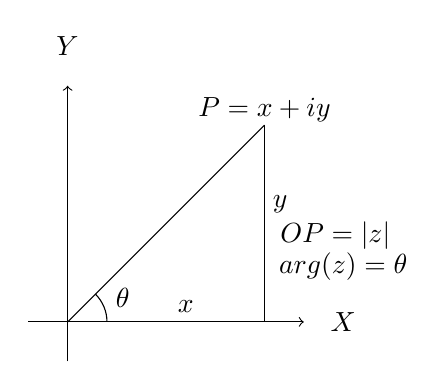
\begin{tikzpicture}
      \draw[->] (-.5,0) -- (3,0);
      \draw[->] (0,-.5) -- (0,3);
      \draw (0, 3.5) node {$Y$};
      \draw (3.5, 0) node {$X$};
      \draw (2.5,0) -- (2.5,2.5);
      \draw (0,0) -- (2.5, 2.5);
      \draw (.5,0) arc(0:45:.5);
      \draw (.7,.3) node{$\theta$};
      \draw (1.5, 0.2) node {$x$};
      \draw (2.7, 1.5) node {$y$};
      \draw (3.4, 1.1) node {$OP=|z|$};
      \draw (3.5, 0.7) node {$arg(z)=\theta$};
      \draw (2.5, 2.7) node{$P=x+iy$};
    \end{tikzpicture}
    \caption{Complex number in argand plane or complex plane}
  \end{center}
\end{figure}

In the diagram, $\theta$ is known as the \textit{argument} of $z$. This is nothing but angle made with positive direction
(i.e. counter-clockwise) of real axis. Now, this argument is not unique. If $\theta$ is an argument of a complex number $z$ then,
$2n\pi + theta$, where $n\in I$, where I is the set of integers. The value of argument for which $-\pi<\theta\leq \pi$ is called
the \textit{principal value} of \textit{argument} or \textit{principal argument}.

\subsection{Different Arguments of a Complex Number}
In the diagram, the argument is given as $\arg(z) = \tan^{-1}\left(\frac{y}{x}\right)$, this value is for when $z$ in first
quadrant. When $z$ will lie in second, third and fourth quadrants the arguments will be
$$\arg(z) = \pi - \tan^{-1}\left(\frac{y}{|z|}\right), arg(z)= -\pi + \tan^{-1}\left(\frac{|y|}{|z|}\right)\text{~and~} arg(z) =
-\tan^P{-1}\left(\frac{|y|}{x}\right)$$
respecticely.

\subsection{Polar Form of a Complex Number}
If $z$ is a non-zero complex number, then we can write $z = r(\cos\theta + i\sin\theta)$, where $r = |z|$ and $\theta = arg(z)$.

In this case, $z$ is also given by $z = r[\cos(2n\pi  \theta) + i\sin(2n\pi + \theta)]$, where $n\in I$.

\subsubsection{Euler's Formula}
The complex number $\cos\theta + i\sin\theta$ is denoted by $e^{i\theta}$ or $c$ is $\theta$, where $c$ is the complex number.

\subsection{Important Results Involving Arguments}
If $z, z_1$ and $z_2$ are complex numbers, then

\begin{enumerate}
\item $arg(\overline{(z)}) = -arg(z)$. This can be easily proven as if $z = x + iy$, then $\overline{z} = x - iy$ i.e. sign of
  argument will get a -ve sign as $y$ gets one.
\item $arg(z_1z_2) = arg(z_1)  + arg(z_2) + 2n\pi$, where
  $$n = \begin{cases}
   0 \text{~if~} & -\pi<arg(z_1)+arg(z_2)\leq-\pi\\
   1 \text{~if~} & -2\pi<arg(z_1)+arg(z_2)\leq-\pi\\
   -1 \text{~if~} & -\pi<arg(z_1)+arg(z_2)\leq2\pi\end{cases}$$
 \item Similarly, $arg(z_1\overline{z_2}) = arg(z_1) - arg(z_2)$.
 \item $|z_1 + z_2| = |z_2 - z_2| \Leftrightarrow arg(z_1) - arg(z_2) = \pi/2$.
 \item $|z_1 + z_2| = |z_1| + |z_2| \Leftrightarrow arg(z_1) = arg(z_2)$.
 \item $|z_1 + z_2|^2 = r_1^2 + r_2^2 + 2r_1r_2\cos(\theta_1 - \theta_2)$.
 \item $|z_1 - z_2|^2 = r_1^2 +r_2^2 + 2r_1r_2\cos(\theta_1 + \theta_2)$.
\end{enumerate}

\section{Vector Representation}
Complex numbers can also be represented as vectors. Length of the vector is nothing but modulus of complex number and argument is
the angle which the vector makes with read axis. It is denoted as $\overrightarrow{OP}$, where $OP$ represents the vector of the
complex number $z$.

\section{Algebraic Operation's Representation}
Let $z_1 = x_1 + iy_1$ and $z_2 = x_2 + iy_2$ be two complex numbers, which are represented by two point $P_1$ and $P_2$ in the
following diagrams.

\subsection{Addition}
Now, as we know that $z_1 + z_2 = (x_1 + x_2) + i(y_1 + y_2)$. Let us see how it looks using geometrically:
\begin{figure}[h]
  \begin{center}
    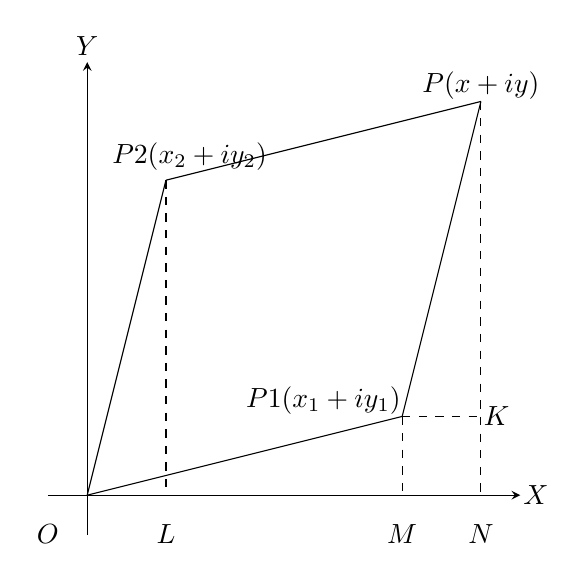
\begin{tikzpicture}
      \draw[->, >=stealth] (-.5,0) -- (5.5,0);
      \draw[->, >=stealth] (0,-.5) -- (0,5.5);
      \draw (5.7, 0) node {$X$};
      \draw (0,5.7) node {$Y$};
      \draw (0,0) -- (4,1);
      \draw (0,0) -- (1,4);
      \draw (1,4) -- (5,5);
      \draw (4,1) -- (5,5);
      \draw[dashed] (4,1) -- (4,0);
      \draw[dashed] (1,4) -- (1,0);
      \draw[dashed] (5,5) -- (5,0);
      \draw[dashed] (4,1) -- (5,1);
      \draw (-.5,-.5) node {$O$};
      \draw (1,-.5) node {$L$};
      \draw (4,-.5) node {$M$};
      \draw (5,-.5) node {$N$};
      \draw (5.2,1) node {$K$};
      \draw (3, 1.2) node {$P1(x_1+iy_1)$};
      \draw (1.3, 4.3) node {$P2(x_2+iy_2)$};
      \draw (5, 5.2) node {$P(x+iy)$};
    \end{tikzpicture}
    \caption{Complex numbers addition}
  \end{center}
\end{figure}
Clearly, $z = z_1 + z_2 = x_1 + x_2 + i(y_1 + y_2)$. Let $P_1M, P_2L$ and $PN$ be parallel to the $y$-axis; $P_1K$ be parallet to
the $x$-axis. This implied that triangle $OP_2L$ and $PP_1K$ are congruent.

We have $P_1K = OL = x_1$ and $P_2L = PK = y_1$

Thus, $ON = OM + MN = OL + P_1K = x_1 + x_2$ and $PN = PK + KN = P_2L + P_1M = y_2 + y_1$

So we can say that coordinates of $P$ are $(x_1 + x_2, y_1 + y_2)$ which represents the complex number $z.$

We also see that this obeys vector addition i.e. $OP_1 + OP_2 = OP_1 + P_1P = OP$

\subsection{Subtraction}
\begin{figure}[h]
  \begin{center}
    \includegraphics{complex-numbers-subtraction}
    \caption{Complex numbers subtraction}
    \label{fig:cns}
  \end{center}
\end{figure}
In figure \ref{fig:cns}, we first represent $-z_2$ by $P_2'$ so that  $P_2P_2'$ is bisected at $O.$ Complete the parallelogram $OP_1PP_2'.$ Then it can be
easily seen that $P$  representd the difference $z_1 - z_2.$

As $OP_1PP_2'$ is a parallelogram so $P_1P = OP_2'.$ Using vetor notation, we have, $z_1 - z_2 = OP_1 - OP_2 = OP_1 + OP_2' = OP_1 + P_1P = P_2P1$

It follows that the complex number $z_1 - z_2$ is represented by the vector $P_1P_2,$ where points $P_1$ and $P_2$ represent the
complex numbers $z_1$ and $z_2$ respectively.

It should be noted that $arg(z_1 - z_2)$ is the angle through which $OX$ must be rotated in the anticlockwise direction to make it
parallel with $P_1P_2.$

\subsection{Multiplication}
\begin{figure}[H]
  \begin{center}
    \includegraphics{complex-numbers-multiplication}
    \caption{Complex numbers multiplication}
  \end{center}
\end{figure}
For multiplication it is convenient to use Euler's formula of complex numbers.

Let $z_1 = r_1e^{i\theta_1}$ and $z_2 = r_2e^{i\theta_2},$ then clealry, $z_1z_2 = r_1r_2e^{i(\theta_1 + \theta_2)}$

\subsection{Division}
\begin{figure}[!h]
  \begin{center}
    \includegraphics{complex-numbers-division}
    \caption{Complex numbers division}
  \end{center}
\end{figure}
For division also it is convenient to use Euler's formula of complex numbers.\\

Let $z_1 = r_1e^{i\theta_1}$ and $z_2 = r_2e^{i\theta_2},$ then clealry, $z_1/z_2 = r_1/r_2e^{i(\theta_1 - \theta_2)}$

\section{Three Important Results}
\begin{figure}[!h]
  \begin{center}
    \includegraphics{complex-numbers-external-angle}
    \caption{External angle}
  \end{center}
\end{figure}
$z_1 - z_2 = \overrightarrow{OP} - \overrightarrow{OQ} = \overrightarrow{QP}$

$\therefore |z_1 - z_2| = |\overrightarrow{QP}| = QP$ which is nothing but distance between $P$ and $Q.$

$arg(z_1 - z_2)$ is the angle made by $\overrightarrow{QP}$ with $x$-axis whis is nothing but $\theta.$
\begin{figure}[h]
  \begin{center}
    \includegraphics{angle-three-complex-numbers}
    \caption{Angle relation between three complex numbers}
    \label{fig:arbtcn}
  \end{center}
\end{figure}

In figure \ref{fig:arbtcn}, $\theta = \alpha - \beta = arg(z_3 - z_1) - arg(z_2 - z_1) \Rightarrow \theta = arg\frac{z_3 - z_1}{z_2 - z_1}$

Similarly if three complex numbers are vertices of a triangle then angles of those vertices can also be computed using previous
results.

Similarly, for four points to be concyclic where those points are represented by $z_1, z_2, z_3$ and $z_4$ if
$$arg\left(\frac{z_2 - z_4}{z_1 - z_4}.\frac{z_1 - z_3}{z_2 - z_4}\right) = 0$$

\section{More Roots}
\subsection{Any Root of an Complex Number is a Complex Number}
Let $x + iy$ be a complex number, where $y \neq 0$.

Let $(x +iy)^n = a\therefore x + iy = a^n$

Now, if $a$ is real, $a^n$ will also be real but from above a complex number $x + iy$ is equal to a real number, $a^n$, which is
not possible. Hence, it must be complex.

\subsection{Square Root of a Complex Number}
Consider a complex number $z = x + iy$. Let $a + ib$ be its square root. Then
$$\sqrt{x + iy} = a + ib \Rightarrow x + iy = (a^2 - b^2) + 2abi$$
Equating real and imaginary parts
$$x = a^2 - b^2, y = 2ab \Rightarrow (a^2 + b^2)^2 = (a^2 - b^2)^2 + (2ab)^2$$
From these two equations, we have
$$a = \pm\sqrt{\frac{\sqrt{x^2 + y^2} + x}{2}}, b = \sqrt{\frac{\sqrt{x^2 - y^2} - x}{2}}$$
\subsection{Cube Roots of Unity}
Let $x = \sqrt[3]{1} \Rightarrow x^3 - 1 = 0$

$\Rightarrow (x - 1)(x^2 + x + 1 ) = 0$

So the three roots are $x = 1, \frac{-1 \pm \sqrt{3}}{2}$ i.e. $1, \frac{-1\pm \sqrt{3}i}{2}$.

It can be easily verified that if $\omega = \frac{-1 -\sqrt{3}i}{2}$, then $\omega^2 = \frac{-1 + \sqrt{3}i}{2}$, thus, three cube
roots are represented as $1, \omega$ and $\omega^2$. $\omega$ is the symbol used for representing cube root of unity.
\subsection{$n$th Root of Unity}
$1 = \cos0 + i\sin 0 \Rightarrow \sqrt[n]{1} = \sqrt[n]{\cos0 + i\sin0}$

\noindent $=\cos\frac{2k\pi}{n} + i\sin\frac{2k\pi}{n}, \text{~where~} k = 0, 1, 2, 3, 4, \ldots (n - 1)$

\noindent $= e^{\frac{2k\pi}{n}} = 1, e^{\frac{i2\pi}{n}}, e^{\frac{i4\pi}{n}}, \ldots, e^{\frac{i2(n - 1)\pi}{n}} = 1, \alpha, \alpha^2,
\ldots, \alpha^{n - 1}, \text{~where~}\alpha = e^{\frac{i2\pi}{n}}$

\noindent Similar to cube roots of unity it can be proven that $1 + \alpha + \alpha^2 + \ldots + \alpha^{n - 1} = 0$
and $1.\alpha.\alpha^2.\ldots\alpha^{n - 1} = (-1)^{n - 1}$

\section{De Moivre's Theoremm}
This theorem's proof uses mathematical induction, so read the chapter on it.

\noindent\textbf{Statement:} If $n$ is any integer then $(\cos\theta + i\sin\theta)^n = \cos n\theta + i\sin n\theta$.

\noindent\textbf{Proof: Case I.} When $n$ is $0$. Clearly, $(\cos\theta + i\sin\theta)^0 = 1$

\noindent\textbf{Case II.} When $n$ is a positive integer. Clearly is it true for $n = 1$

\noindent Let it is true for $n = m$. Then $(\cos\theta + i\sin\theta)^m = \cos m\theta + i\sin m\theta$

\noindent For $n = m + 1, (\cos\theta + i\sin\theta)^{m + 1} = (\cos m\theta + i\sin m\theta)(\cos\theta + i\sin\theta) = \cos(m + 1)\theta +
i\sin(m + 1)\theta$ [this result comes from trigonometry]

\noindent Thus, by mathematical induction we have proven the theorem for positive integers.

\noindent\textbf{Case III.} When $n$ is negative number. For $n = -1, (\cos\theta + i\sin\theta)^{-1} = \frac{1}{\cos\theta +
  i\sin\theta}$

\noindent $= \frac{\cos\theta - \i\sin\theta}{\cos^2\theta + \sin^2\theta} = \cos\theta - i\sin\theta$

\noindent Let it be true for $n = -m, (\cos\theta + i\sin\theta)^{-m} = \cos m\theta - i\sin m\theta$

\noindent For $n = -(m + 1), (\cos\theta + i\sin\theta)^{-(m + 1)} = \frac{\cos m\theta - i\sin m\theta}{\cos\theta + i\sin\theta}$

\noindent $= (\cos m\theta - i\sin m\theta)(\cos\theta - i\sin\theta) = \cos(m + 1)\theta + i\sin(m + 1)\theta$

Thus, it is proven for negative numbers as well. Proof for fractional powers is left as an exercise.

\section{Some Important Geometrical Results}
\subsection{Section Formula}
Let $z_1 = x_1 + iy_1, z_2 = x_2 + iy_2$ then $z = x + iy$, which divides the previous two points in the ratio m;nm;n can be given
by using the results from coordinate geometry as below:
$$x = \frac{mx_2 + nx_1}{m + n}, y = \frac{my_2 + ny_1}{m + n} \text{~and~}z = \frac{mz_2 + nz_1}{m + n}$$
Extending this section formula, we can say that if there is a point which is mid-point i.e. divides a line in two equal parts, then
$m = 1$ and $n = 1$ then $z$ is given by $\frac{1}{2}(z_1 + z_2)$.
\subsection{Distance Formula}
Distance between $A(z_1)$ and $B(z_2)$ is given by $AB = |z_1 - z_2|$.
\subsection{Equation of a Line}
The equation between two points $z_1$ and $z_2$ is given by the determinant
$$\begin{vmatrix}z&\overline{z}&1\\z_1&\overline{z_1}&1\\z_2&\overline{z_2}&1\end{vmatrix} = 0$$
or,
$$\frac{z - z_1}{\overline{z} - \overline{z_1}} = \frac{z_1 - z_2}{\overline{z_1} - \overline{z_2}}$$
The parametric form is given by $z = iz_1 + (1 - t)z_2$
\subsection{Collinear Points}
Three points $z_1, z_2$ and $z_3$ are collinear if and only if
$$\begin{vmatrix}z_1&\overline{z_1}&1\\z_2&\overline{z_2}&1\\z_3&\overline{z_3}&1\end{vmatrix} = 0$$
\subsection{Parallelogram}
Four complex numbers $A(z_1), B(z_2), C(z_3)$ and $D(z_4)$ represent the vertices of a parallelogram if $z_1 + z_3 = z_2 +
z_4$.This result comes from the fact that diagonals of a parallelogram bisect each other.
\begin{figure}[h]
  \begin{center}
    \includegraphics{complex-number-parallelogram}
    \caption{Parallelogram}
  \end{center}
\end{figure}
\subsection{Rhombus}
Four complex numbers $A(z_1), B(z_2), C(z_3)$ and $D(z_4)$ represent the vertices of a rhombus if $z_1 + z_3 = z_2 + z_4$ and
$|z_4 - z_1| = |z_2 - z_1|$.
\begin{figure}[h]
  \begin{center}
    \includegraphics{complex-number-rhombus}
    \caption{Rhombus}
  \end{center}
\end{figure}
The diagonals must bisect each other. Thus, $z_1 + z_3 = z_2 + z_4.$ Also, four sides of a rhombus are equal i.e. $AD = AB
\Rightarrow |z_4 - z_1| = |z_2 - z_1|$.

\subsection{Square}
Four complex numbers $A(z_1), B(z_2), C(z_3)$ and $D(z_4)$ represent the vertices of a square if $z_1 + z_3 = z_2 + z_4,
|z_4 - z_1| = |z_2 - z_1|$ and $|z_3 - z_1| = |z_4 - z_2|$.
\begin{figure}[h]
  \begin{center}
    \includegraphics{complex-number-square}
    \caption{Square}
  \end{center}
\end{figure}

The diagonals must bisect each other. Thus, $z_1 + z_3 = z_2 + z_4.$ Also, four sides of a square are equal i.e. $AD = AB
\Rightarrow |z_4 - z_1| = |z_2 - z_1|$.

Also the digonals are equal in length so $|z_3 - z_1| = |z_4 - z_2|$.

\subsection{Rectangle}
Four complex numbers $A(z_1), B(z_2), C(z_3)$ and $D(z_4)$ represent the vertices of a square if $z_1 + z_3 = z_2 + z_4$ and $|z_3
- z_1| = |z_4 - z_2|$.
\begin{figure}[h]
  \begin{center}
    \includegraphics{complex-number-rectangle}
    \caption{Rectangle}
  \end{center}
\end{figure}

The diagonals must bisect each other. Thus, $z_1 + z_3 = z_2 + z_4$. Also, the digonals are equal in length so $|z_3 - z_1| = |z_4
- z_2|$.

\subsection{Centroid of a Triangle}
Let $A(z_1), B(z_2)$ and $C(z_3)$ be the vertices of a $\triangle ABC.$ Centroid $G(z)$ of the $\triangle ABC$ is the point of
concurrence of the medians of all three sides and is given by
$$z = \frac{z_1 + z_2 + z_3}{3}$$
\begin{figure}[h]
  \begin{center}
    \includegraphics{complex-number-centroid}
    \caption{Centroid of a Triangle}
  \end{center}
\end{figure}

\subsection{Incenter of a Triangle}
Let $A(z_1), B(z_2)$ and $C(z_3)$ be the vertices of a $\triangle ABC.$ inceneter $I(z)$ of the $\triangle ABC$ is the point of
concurrence of the internal bisectors of and is given by
$$z = \frac{az_1 + bz_2 + cz_3}{a + b + c}$$
where $a, b, c$ are the lengths of the sides.

\subsection{Circumcenter of a Triangle}
Circumcenter $S(z)$ of a $\triangle ABC$ is the point of concurrence of perpendicular bisectors of sides of the triangle. It is
given by

$$z = \frac{(z_2 - z_3)|z_1|^2 + (z_3 - z_1)|z_2|^2 + (z_1 - z_2)|z_3|^2}{\overline{z_1}(z_2 - z_3) + \overline{z_2}(z_3 - z_1) + \overline{z_3}(z_1 - z_2)}$$
$$= \frac{\begin{vmatrix}|z_1|^2 & z_1 & 1\\ |z_2|^2 & z_2 & 1 \\ |z_3|^2 & z_3 & 1\end{vmatrix}}{\begin{vmatrix}\overline{z_1} & z_1 & 1\\\overline{z_2} & z_2 & 1\\\overline{z_3} & z_3 & 1 \end{vmatrix}}$$
Also,
$$z = \frac{z_1\sin2A + z_2\sin2B + z_3\sin2C}{\sin2A + \sin2B + \sin2C}$$

\subsection{Orthocenter of a Triangle}
The orthocenter $H(z)$ of the $\triangle ABC$ is the point of concurrence of altitudes of the side. It is given by
$$z = \frac{\begin{vmatrix}z_1^2 & \overline{z_1} & 1\\z_2^2 & \overline{z_2} & 1\\z_3^2 & \overline{z_3} & 1\end{vmatrix} + \begin{vmatrix}|z_1|^2 & z_1 & 1\\|z_2|^2 & z_2 & 1\\|z_3|^2 & z_3 & 1\end{vmatrix}}{\begin{vmatrix}\overline{z_1} & z_1 & 1\\\overline{z_2} & z_2 & 1\\\overline{z_3} & z_3 & 1\end{vmatrix}}$$
$$= \frac{z_1\tan A + z_2\tan B + z_3\tan C}{\tan A + \tan B + \tan C}$$
$$= \frac{z_1a\sec A + bz_2\sec B + cz_3\sec C}{a\sec A + b\sec B + c\sec C}$$

\subsection{Euler's Line}
The centroid $G$ of a triangle lies on the segment joining the orthocenter $H$ and the circumcenter $S$ of the triangle. $G$
divides the line $H$ and $S$ in the ratio $2:1$.

\subsection{Length of Perpendicular from a Point to a Line}
Length of a perpendicular of point $A(\omega)$ from the line $\overline{a}z + a\overline{z} + b = 0, (a\in C, b\in R)$
is given by

$$p = \frac{|\overline{a}\omega + a\overline{\omega} + b|}{2|a|}$$

\subsection{Equation of a Circle}
The equation of a circle with center $z_0$ and radius $r$ is $|z- z_0| = r$ or $z = z_0 + re^{i\theta}, 0\leq \theta\leq 2\pi$ or
$z\overline{z} - z_0\overline{z} - \overline{z_0}z + z_0\overline{z_0} - r^2 = 0$

\noindent General equation of a circle is $z\overline{z} - a\overline{z} + \overline{a}z + b = 0, (a\in C, b\in R)$ such that $\sqrt{a\overline{a} - b}\geq 0.$

\noindent Center of this circle is $-a$ and radius is $a\overline{a} - b.$

\noindent An equation of the circle, one of whose diameter is the line segment joining $z_1$ and $z_2$ is $(z - z_1)(\overline{z} - \overline{z_2}) + (\overline{z} - \overline{z_1})(z - z_2) = 0$

\noindent An equation of the the circle passing through two points $z_1$ and $z_2$ is
$$(z - z_1)(\overline{z} - \overline{z_2}) + (\overline{z} - \overline{z_1})(z - z_2) + k \begin{vmatrix}z & \overline{z} & 1\\z_1
  & \overline{z_1} & 1\\z_2 & \overline{z_2} & 1 \end{vmatrix} = 0$$
where $k$ is a parameter.

\subsection{Equation of a Circle Passing through Three Points}
\begin{figure}[h]
  \begin{center}
    \includegraphics{complex-number-circle}
    \caption{Circle through three points}
  \end{center}
\end{figure}
We choose any point $P(z)$ on the circle. Two such points are shown in the figure above one is in same segment with $C$
and the other one in different segement. So we have
$$\angle ACB = \angle APB\text{~or~}\angle ACB + \angle APB = \pi$$
$$\arg\frac{z_3 - z_2}{z_3 - z_1} - arg\frac{z - z_2}{z - z_1} = 0\text{~or~}\arg\frac{z_3 - z_2}{z_3 - z_1} + arg\frac{z - z_2}{z - z_1} = \pi$$
Clearly, in both cases the fraction must be purely real. Thus we can apply the property of conjugates i.e. $z = \overline{z}$ which
also gives us the condition for four concyclic points.

$$\Rightarrow \frac{(z - z_1)(z_3 - z_2)}{(z - z_2)(z_3 - z_1)} = \frac{\overline{(z - z_1)(z_3 - z_2)}}{\overline{(z - z_2)(z_3 -
    z_1)}}$$
From this we can also deduce the condition for four points to be concyclic. Treating $P(z)$ as just another point $D(z_4)$, we can
rewrite the abobe result as
$$\frac{(z_4 - z_1)(z_3 - z_2)}{(z_4 - z_2)(z_3 - z_1)} = \frac{\overline{(z_4 - z_1)(z_3 - z_2)}}{\overline{(z_4 -
    z_2)(z_3 - z_1)}}$$

\subsection{Finding Loci by Examination}
\begin{enumerate}
\item $\arg(z - z_0) = \alpha$

  If $\alpha$ is a real number and $z_0$ is a fixed point, then $\arg(z - z_0) =\alpha$ represents a vector starting at
  $z_0$(exlcluding  the point $z_0$) and making an angle $\alpha$ with real $x$-axis.
  \begin{figure}[h]
    \begin{center}
      \includegraphics{complex-number-loci1}
    \end{center}
  \end{figure}

  Now suppose $z_0$ is origin $O$, then the above equation becomes $\arg(z) = \alpha$, which is a vector starting at origin and
  making an angle $\alpha$, which is a vector starting at origin and making an angle $\alpha$ with $x$-axis.
\item If $z_1$ and $z_2$ are two fixed points such that $|z - z_1| = |z - z_2|$ then $z$ represents perpendicular bisector of the
  segment joining $A(z_1)$ and $B(z_2).$ And $z, z_1, z_2$ will form an isoscles triangle.
  \begin{figure}[h]
    \begin{center}
      \includegraphics{complex-number-loci2}
    \end{center}
  \end{figure}

  If $z_1$ and $z_2$ are two fixed points and $k > 0, k\neq 1$ is a real number then $\frac{|z- z_1|}{|z - z_2|} = k$ represents a
  circle.
\item $|z - z_1| + |z - z_2| = k$. Let $z_1$ and $z_2$ be two fixed points and $k$ be a positive real number.
  \begin{enumerate}
    \item Refer figure \ref{fig:flbee}, if $k > |z - z_2|,$ then $|z - z_1| + |z - z_2| = k$ represents an ellipse with foci at $A(z_1)$ and $B(z_2)$ and length
      of major axis $= k$.
      \begin{figure}[h]
        \begin{center}
          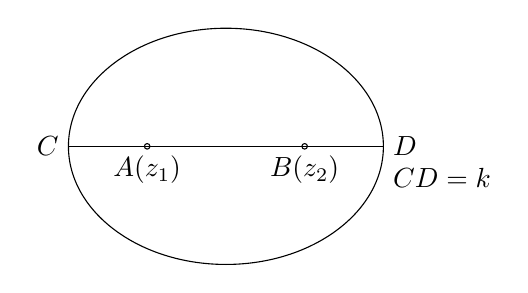
\begin{tikzpicture}
            \draw (0, 0) ellipse (2 and 1.5);
            \draw (-2, 0) node[anchor=east] {$C$} (2, 0) node[anchor=west] {$D$};
            \draw (-2, 0) -- (2, 0);
            \draw (-1, 0) node[anchor=north] {$A(z_1)$} (1, 0)
            node[anchor=north] {$B(z_2)$};
            \draw (-1, 0) circle(1pt) (1, 0) circle(1pt) (2, -.4)
            node[anchor=west] {$CD = k$};
          \end{tikzpicture}
          \caption{\label{fig:flbee}Locus of an Ellipse}
        \end{center}
      \end{figure}
    \item If $k = |z - z_2|$, then it represents the line segment joining $z_1$ and $z_2$.
    \item If $k < |z - z_2|$, thne it does not represent any curve/line in Argand plane.
  \end{enumerate}
\item If $|z - z_1| - |z - z_2| = k$. Let $z_1$ and $z_2$ be two fixed points and $k$ be a positive real number.
  \begin{enumerate}
  \item Refer figure \ref{fig:flbep}, if $k\neq |z - z_2|$, then it represnts a parabola with foci at $A(z_1)$ and $B(z_2)$.
    \begin{figure}[H]
      \begin{center}
        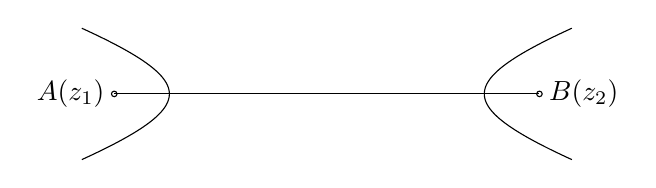
\begin{tikzpicture}
          \draw plot[variable=\t,samples=100,domain=-50:50]
          ({2*sec(\t)},{.7*tan(\t)});
          \draw plot[variable=\t,samples=100,domain=-50:50]
          ({-2*sec(\t)},{.7*tan(\t)});
          \draw (-2.7,0) -- (2.7, 0);
          \draw (-2.7, 0) circle(1pt) (2.7, 0) circle(1pt);
          \draw (-2.7, 0) node[anchor=east] {$A(z_1)$} (2.7, 0)
          node[anchor=west] {$B(z_2)$};
        \end{tikzpicture}
        \caption{\label{fig:flbep} Locus of a parabola}
      \end{center}
    \end{figure}
    \item If $k = |z_1 - z_2|$, then it represents the straight line joining $A(z_1)$ and $B(z_2)$ but excluding the segment $AB$
      \begin{figure}[H]
        \begin{center}
          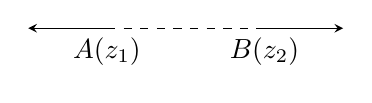
\begin{tikzpicture}
            \draw[dashed] (-1, 0) -- (1, 0);
            \draw[->, >= stealth] (-1, 0) -- (-2, 0);
            \draw[->, >= stealth] (1, 0) -- (2, 0);
            \draw (-1, 0) node[anchor=north] {$A(z_1)$} (1, 0) node[anchor=north] {$B(z_2)$};
          \end{tikzpicture}
        \end{center}
      \end{figure}
  \end{enumerate}
  \item $|z - z_1|^2 + |z - z_2|^2 = |z_1 - z_2|^2$. If $z_1$ and $z_2$ are two fixed points then it represents a circle with $z_1$
    and $z_2$ as the endpoints of one of the diameters.
    \begin{figure}[H]
      \begin{center}
        \begin{tikzpicture}
          \draw (0, 0) circle(2);
          \draw (-2, 0) -- (2, 0) (-2, 0) node[anchor=east] {$A(z_1)$}
          (2, 0) node[anchor=west] {$B(z_2)$};
          \draw (0, 0) circle(1pt) (0,0) node[anchor=north] {$O$};
        \end{tikzpicture}
      \end{center}
    \end{figure}
  \item $\arg\left(\frac{z - z_1}{z - z_2}\right) = \alpha$. Let $z_1$ and $z_2$ be any two fixed points and $\alpha$ be a real
    number such that $0\leq \alpha \leq \pi$.
    \begin{enumerate}
    \item If $0 < \alpha < \pi$ and $\alpha \neq \pi/2$, then it represents a segment of a circle passing through $A(z_1)$ and
      $B(z_2)$.
      \begin{figure}[H]
        \begin{center}
          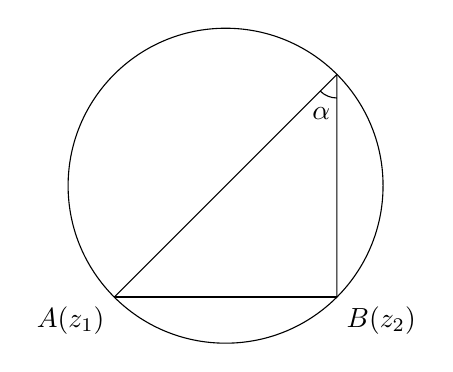
\begin{tikzpicture}
            \draw (0, 0) circle(2);
            \draw (-1.414, -1.414) -- (1.414, -1.414);
            \draw (-1.414, -1.414) -- (1.414, 1.414) (1.414, -1.414) -- (1.414,
            1.414);
            \draw (1.414, 1.114) arc(270:225:.3);
            \draw (-1.414, -1.414) node[anchor=north east] {$A(z_1)$} (1.414,
            -1.414) node[anchor=north west] {$B(z_2)$};
            \draw (1.214, 1.114) node[anchor=north] {$\alpha$};
          \end{tikzpicture}
        \end{center}
      \end{figure}
    \item If $\alpha = \pi/2$, then it represents a circle with diameter as the line segment joining $A(z_1)$ and $B(z_2)$.
      \begin{figure}[H]
        \begin{center}
          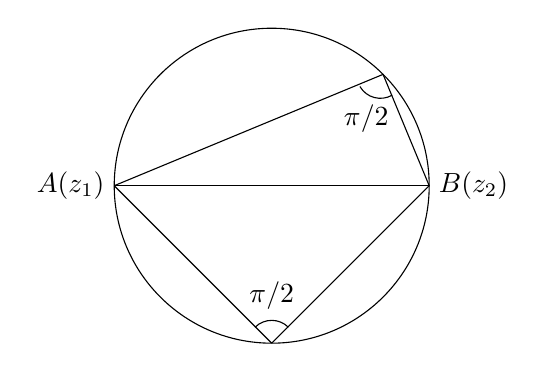
\begin{tikzpicture}
            \draw (0, 0) circle(2);
            \draw (-2, 0) -- (2, 0);
            \draw (-2, 0) -- (1.414, 1.414) (2, 0) -- (1.414, 1.414) (-2, 0) --
            (0, -2) (2, 0) -- (0, -2);
            \draw (-2, 0) node[anchor=east] {$A(z_1)$} (2,
            0) node[anchor=west] {$B(z_2)$};
            \draw (1.53, 1.15) arc(300:210:.3);
            \draw(.2121, -1.7979) arc(45:135:.3);
            \draw (1.2, 1.15) node[anchor=north] {$\pi/2$} (0, -1.7)
            node[anchor=south] {$\pi/2$};
          \end{tikzpicture}
        \end{center}
      \end{figure}
    \item If $\alpha = \pi$, then it represents the straight line joining $A(z_1)$ and $B(z_2)$ but excluding the line segment $AB$.
      \begin{figure}[H]
        \begin{center}
          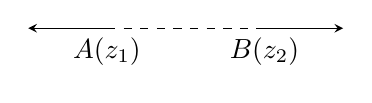
\begin{tikzpicture}
            \draw[dashed] (-1, 0) -- (1, 0);
            \draw[->, >= stealth] (-1, 0) -- (-2, 0);
            \draw[->, >= stealth] (1, 0) -- (2, 0);
            \draw (-1, 0) node[anchor=north] {$A(z_1)$} (1, 0) node[anchor=north] {$B(z_2)$};
          \end{tikzpicture}
        \end{center}
      \end{figure}
    \item If $\alpha = 0,$ then it represents the straight line joining $A(z_1)$ and $B(z_2)$.
      \begin{figure}[H]
        \begin{center}
          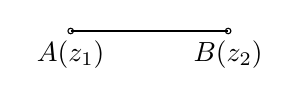
\begin{tikzpicture}
            \draw (-1, 0) -- (1, 0);
            \draw (-1, 0) node[anchor=north] {$A(z_1)$} (1, 0) node[anchor=north] {$B(z_2)$};
            \draw (-1, 0) circle(1pt) (1, 0) circle(1pt);
          \end{tikzpicture}
        \end{center}
      \end{figure}
    \end{enumerate}
\end{enumerate}
\section{Problems}
Find the square root of the following complex numbers:

\begin{enumerate}
  \item $7 + 8i$
\end{enumerate}
